%%%%%%%%%%%%%%%%%%%%%%%%%%%%%%%%%%%%%%%%%%%%%%%%%%%%%%%%%%%%%%%%
% %
% Seth Cram %
% ECE351 Section 53 %
% Lab 7 %
% Due 03/08/2022 %
% Any other necessary information needed to navigate the file %
%
%
% %
%%%%%%%%%%%%%%%%%%%%%%%%%%%%%%%%%%%%%%%%%%%%%%%%%%%%%%%%%%%%%%%%
%%%%%%%%%%%%%%%%%%%%%%%%%%%%%%%%%%%%%%%%%%%
%%% DOCUMENT PREAMBLE %%%
\documentclass[12pt]{report}
\usepackage[english]{babel}
%\usepackage{natbib}
\usepackage{url}
\usepackage[utf8x]{inputenc}
\usepackage{amsmath}
\usepackage{graphicx}
\graphicspath{{images/}}
\usepackage{parskip}
\usepackage{fancyhdr}
\usepackage{vmargin}
\usepackage{listings}
\usepackage{hyperref}
\usepackage{xcolor}
\usepackage{verbatim}
\usepackage{listings}

\definecolor{codegreen}{rgb}{0,0.6,0}
\definecolor{codegray}{rgb}{0.5,0.5,0.5}
\definecolor{codeblue}{rgb}{0,0,0.95}
\definecolor{backcolour}{rgb}{0.95,0.95,0.92}

\begin{comment} %have to use verbatim package for this

\section{Personal Notes}
            


\end{comment}

\lstdefinestyle{mystyle}{
    backgroundcolor=\color{backcolour},   
    commentstyle=\color{codegreen},
    keywordstyle=\color{codeblue},
    numberstyle=\tiny\color{codegray},
    stringstyle=\color{codegreen},
    basicstyle=\ttfamily\footnotesize,
    breakatwhitespace=false,         
    breaklines=true,                 
    captionpos=b,                    
    keepspaces=true,                 
    numbers=left,                    
    numbersep=5pt,                  
    showspaces=false,                
    showstringspaces=false,
    showtabs=false,                  
    tabsize=2
}
 
\lstset{style=mystyle}

\setmarginsrb{3 cm}{2.5 cm}{3 cm}{2.5 cm}{1 cm}{1.5 cm}{1 cm}{1.5 cm}

\title{Lab 7}		%TITLE						
% Title
\author{ Seth Cram}						
% Author
\date{03/08/2022}
% Date

\makeatletter
\let\thetitle\@title
\let\theauthor\@author
\let\thedate\@date
\makeatother

\pagestyle{fancy}
\fancyhf{}
\rhead{\theauthor}
\lhead{\thetitle}
\cfoot{\thepage}
%%%%%%%%%%%%%%%%%%%%%%%%%%%%%%%%%%%%%%%%%%%%
\begin{document}

%%%%%%%%%%%%%%%%%%%%%%%%%%%%%%%%%%%%%%%%%%%%%%%%%%%%%%%%%%%%%%%%%%%%%%%%%%%%%%%%%%%%%%%%%

\begin{titlepage}
	\centering
    \vspace*{0.5 cm}
   % \includegraphics[scale = 0.075]{bsulogo.png}\\[1.0 cm]	% University Logo
\begin{center}    \textsc{\Large   ECE 351 - 53 }\\[2.0 cm]	\end{center}% University Name
	\textsc{\Large Block Diagrams and System Stability }\\[.5 cm]				% Course Code
	\rule{\linewidth}{0.2 mm} \\[0.4 cm]
	{ \huge \bfseries \thetitle}\\
	\rule{\linewidth}{0.2 mm} \\[1.5 cm]
	
	\begin{minipage}{0.4\textwidth}
		\begin{flushleft} \large
		%	\emph{Submitted To:}\\
		%	Name\\
          % Affiliation\\
           %contact info\\
			\end{flushleft}
			\end{minipage}~
			\begin{minipage}{0.4\textwidth}
            
			\begin{flushright} \large
			\emph{Submitted By :} \\
			Seth Cram  
		\end{flushright}
           
	\end{minipage}\\[2 cm]
	
\end{titlepage}

%%%%%%%%%%%%%%%%%%%%%%%%%%%%%%%%%%%%%%%%%%%%%%%%%%%%%%%%%%%%%%%%%%%%%%%%%%%%%%%%%%%%%%%%%

\tableofcontents
\pagebreak

%%%%%%%%%%%%%%%%%%%%%%%%%%%%%%%%%%%%%%%%%%%%%%%%%%%%%%%%%%%%%%%%%%%%%%%%%%%%%%%%%%%%%%%%%
\renewcommand{\thesection}{\arabic{section}}

\section{Introduction}

The goal of lab 7 is to become familiar with Laplace-domain block diagram and utilize the already factored form of their transfer function to judge system stability using Python in the Spyder IDE.

\section{Equations}
    \begin{equation}
        G(s) = \frac{s+9}{(s^2-6s-16)(s+4)} = \frac{s+9}{(s-8)(s+2)(s+4)}
    \end{equation}
    
    \begin{equation}
        A(s) = \frac{s+4}{s^2+4s+3} = \frac{s+4}{(s+1)(s+3)}
    \end{equation}
 
     \begin{equation}
        B(s) = s^2+26s+168 = (s+12)(s+14)
    \end{equation}
    
    \begin{equation}
        H_{open}(s) = \frac{s+9}{(s+1)(s+3)(s-8)(s+2)}
    \end{equation}
    
    \begin{equation}
        H_{closed}(s) = \frac{GA}{1+GB} = \frac{(s+9)(s+4)}{[(s-8)(s+2)(s+4) + (s+9)(s+12)(s+14)](s+1)(s+3)} 
    \end{equation}
    
\section{Methodology}

%This section will describe how you went about solving the lab. Make sure you go into detail about any method you used. %Include coding samples here if necessary. This is also where you would include necessary derivations. An example of %inserting code into the report is given. Do not go overboard on inserting code into your report, only use whats %absolutely necessary to illustrate your point.

    \paragraph{} First, I used the given equations for A(s), G(s), and B(s) to find the poles and zeros of each function by-hand. Then, I used the tf2zpk and roots functions from the scipy and numpy modules to verify the poles and zeros I'd found. I then derived the equation for the open-loop transfer function by-hand. I was able to disregard the B(s) functional block in my calculations since it's in a feedback loop. 
    
    \paragraph{} I then explained why the transfer function is unstable in the "Results" section of my report. I used the scipy module's convolution function to expand both the numerator and denominator of the open-loop transfer function. Using the scipy step function, I found and plotted the step response. Then, explained why the resultant plot gave me an exponential curve. 
    
    \paragraph{} In much of the same fashion, I calculated the closed-loop transfer function by-hand, and then explained why it was stable. Using the step response plot, I reaffirmed that the open-loop system is stable. 
    
\section{Results}

%This section will go over the results of the lab. Use this area to describe %if the lab worked as expected or if the results are unexpected or different %from your hand calculations or intuition. Part of being a good engineer is %gaining intuition about these problems and being able to understand quickly %if something is wrong. Use code, plots, tables, and figures as necessary. %Make sure to cite all other works used and note them in the bibliography. A %sample entry is in this document.

    \paragraph{} Considering the three given equations, their corresponding poles and roots are shown below: \\
    G(s): root = -9; poles = 8, -2, -4 \\
    A(s): root = -4; poles = -1, -3 \\
    B(s): roots = -12, -14 \\
    
    Which are verified by the following console output: \\
    \begin{lstlisting}
        G(s)
        zeroes:  [-9.]
        poles:  [ 8. -4. -2.]
        Gain:  1.0

        A(s)
        zeroes:  [-4.]
        poles:  [-3. -1.]
        Gain:  1.0

        B(s)
        zeroes:  [-14. -12.]
    \end{lstlisting}
    
    \paragraph{} Considering equation 4, $H_{open}(s)$, the open-loop response is unstable since there is a pole at s=8 in the right-hand-plane. So, this would produce a discontinuity and the open-loop response must be unstable since it's unstable at a single point in the right-hand-plane. 
    
    \paragraph{} My expectation for the open system's transfer function's step response was that it should have a discontinuity at s=8, but otherwise would be smooth. 
    
    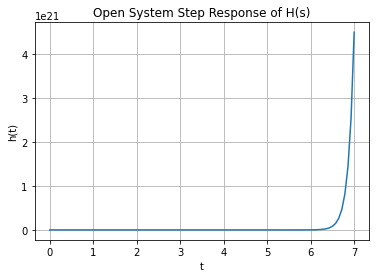
\includegraphics[scale=0.6]{open.png}
    
    \paragraph{} As seen above, my expectations didn't hold true because the step response only plotted until t=7. But, the step response supports my previous assessment that the open-loop response is unstable because a singular value is never converged to on the graph.   
    
    \paragraph{} Considering equation 5, $H_{closed}(s)$, the closed-loop response is stable since the only pole in the right-hand-plane is added to another term in the denominator. The only poles that can zero out the denominator are in the left-hand-plane, -1 and -3, so the open-loop response must be stable. 
    
    \paragraph{} My expectation for the closed system's transfer function's step response was that it shouldn't have any discontinuities. 
    
    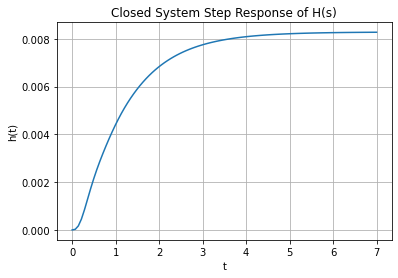
\includegraphics[scale=0.6]{closed.png}
    
    \paragraph{} As seen above, there are no discontinuities because the step response is plotted after t = 0 and none of the poles are in the right hand plane. More telling, we can see how the graph converges on a single point. Therefore, the step response supports my previous assessment that the closed-loop response is stable.   


\section{Error Analysis}

%This section will discuss error analysis of the experiment. Since this lab %deals with ideal simulation there shouldn't be any sources of error, so %instead this section can be used to describe any difficulties you had during %lab and how you solved them. Alternatively, if you couldn't get the %experiment to work, which is okay, you need to use this section to explain why %you couldn't get it to work to earn full points. 

\paragraph{} The main difficulty I encountered was wrapping my head around using the convolution function to expand the numerator and denominator. I'd always previously thought of convolution as a restricted and single use type of function. I can't think of a source of error that might have plagued me during this lab. Our extensive usage of the python functions during the lab helped out in this respect. 

\section{Questions} %also address any deliverables not yet put in yet
    \begin{enumerate}
        \item  In Part 1 Task 5, why does convolving the factored terms using scipy.signal.convolve() result in the expanded form of the numerator and denominator? Would this work with your user-defined convolution function from Lab 3? Why or why not?
        \paragraph{} Because convolution is just multiplying through integration over time, so it makes sense that we'd get the product of two terms convolved together. The reasoning behind this is since we're working in the frequency domain. I assume this would work with my user-defined convolution function from lab3. It's possible that it wouldn't though because the library function does convolution through integration, while ours uses convolution through summation.
        \item Discuss the difference between the open- and closed-loop systems from Part 1 and Part 2. How does stability differ for each case, and why?
        \paragraph{}   The differences between the open and closed loop systems is that we don't consider the negative feedback loops for the open loop system. As a result of this difference, the open loop system is unstable, while the closed loop system is stable. Therefore, negative feedback loops are important for system stability. 
        
        \item What is the difference between scipy.signal.residue() used in Lab 6 and scipy.signal.tf2zpk() used in this lab?
        \paragraph{} The residue function is used to compute partial-fraction expansion of a single expression, while tf2zpk() just factors terms into a single expression. They're pretty specific to these use cases. So, although both functions have the same output of poles, zeros, and gain, they perform different functionality.  
                
        \item Is it possible for an open-loop system to be stable? What about for a closed-loop system to be unstable? Explain how or how not for each
        \paragraph{} Yes, for both. all a system needs to be unstable is a pole in the right hand plane. So, for a closed-loop system this means a single block function without a negative feedback loop and a positive pole in the denominator that doesn't cancel out. The opposite is true for a system that's stable. For an open-loop system, to make it stable we'd just need to make sure none of the blocks contain positive poles in their denominators.    
                
        \item Leave any feedback on the clarity/usefulness of the purpose, deliverables, and expectations for this lab.
        \paragraph{} The goals of the lab, deliverables, and expectations were clear. 
    \end{enumerate}

\section{Conclusion}

%Discuss briefly what you learned in this lab and whether or not you feel the %lab was successful. Include any recommendations for future labs as this is a %learning experience for all of us. Discuss any insights you gained from this %lab and how that will affect future work. \textit{Note: The bibliograhpy %needs to be on its own page.}

    \paragraph{} During lab 7, we analyzed the difference between a closed and open loop version of the same system. We also explored using convolution for expansion purposes. Lab 7 was successful because I became more familiar with Laplace-domain block diagrams and using the factored form of the transfer function to evaluate system stability. The exploration into convolution was an interesting addition.  
    
    Github: \url{https://github.com/SethCram} 

\end{document}